\section{Reaktive Programmierung}
\label{section:reaktive_programmierung}
Reaktive Programmierung ist ein ereignisgesteuertes (event-driven) Programmierparadigma, bei dem der Programmablauf
als Sequenz von asynchronen Ereignissen (Events), und Daten als, von außen unveränderliche (immutable), Datenströme (Streams) dargestellt werden.
Sobald es innerhalb des Datenstroms zu Änderungen kommt werden diese als Events durch einen Publisher veröffentlicht.
Diese Events werden dann von einem oder mehreren \verb|Subscribern| konsumiert. Diese können wiederrum weitere Events durch einen Publisher veröffentlichen.

Die treibende Kraft bzw. der Stimulus von reaktiven Anwendungen sind also interne Änderungen innerhalb der Datenströme, wie beispielsweise das
Hinzufügen eines Elements, welche anschließend den weiteren Programmablauf durch das Auslösen eines Events (durch einen Publisher) starten.

Die Grundidee orientiert sich am Observer-Pattern und dessen Ausprägung dem Publish-Subscribe Pattern, erweitert diese aber
noch um die Benachrichtigungen des Subscribers:
\begin{enumerate}
	\item Sobald keine Events mehr kommen
	\item Wenn ein Fehler aufgetreten ist
\end{enumerate}
Indem Änderungen eines Datenstroms direkt propagiert werden und der Subscriber diesen nicht modifizieren kann, sondern lediglich über Änderungen informiert wird,
können Programme ohne jeglichen Zustand realisiert werden\parencite{Escoffier2017}.

Während ein Datenstrom selber von außen unverändlich ist, kann aber dennoch der Inhalt, also die Daten,
des vom Publisher veröffentlichten Events modifiziert werden, bis es vom
Subscriber konsumiert wird, und zwar in beliebig vielen Schritten.

Für eine solche Verkettung von Verarbeitungsschritten für Events bzw. Daten
wird oft der Begriff \verb|Pipeline| verwendet und jeder Verarbeitungsschritt als \verb|Pipe| bezeichnet.
Durch diese Pipelines \textit{fließen} Elemente in Form von Events bzw. Daten von ihrer Quelle
bis zu einer Senke, dem Ziel bzw. dem eigentlichen Subscriber der \verb|Pipeline|.

Daher wird dieser Prozess auch als \verb|event flow| oder \verb|data flow| bezeichnet.
Jede \verb|Pipe| kann ein Element ändern, löschen oder auch neue Elemente erstellen und dem \verb|flow| hinzufügen.


Allgemein fließt ein Element immer stromabwärts also von der Quelle zur Senke
\footnote{Es gibt aber auch Ausnamefälle in denen ein Element stromaufwärts fließt, also von einer pipe oder von der Senke zur Quelle},
dabei wird die vorherige \verb|pipe| als \verb|upstream| bezeichnet und die nächste, zu durchfließende \verb|pipe| als \verb|downstream|.
Im Hintergrund kommt dabei wieder das Publish-Subscribe Pattern zum Einsatz. Elemente werden von einer durchlaufenen \verb|pipe| als \verb|Publisher|
veröffentlicht und von der nächsten \verb|pipe| als \verb|Subscriber| konsumiert.

Jede \verb|Pipe| kann eine Vielzahl an konkreten Operatoren enthalten die in der jeweiligen Reactive Programming-Bibliothek definiert sind.
Jeder Operator muss dabei wiederrum einen Publisher zur Verfügung stellen, auf den sich der nachfolgende Operator registrieren kann
um die transformierten Elementen zu erhalten.

\footnote{Obwohl die Implementierungsdetails und die verwendete Terminologie unterschiedlich sind, abhängig von der verwendeten Reactive Programming-Bibliothek
	und der Programmiersprache, ist der Arbeitsablauf immer ähnlich}
In Listing \ref{lst:eventflow_pseudocode} wird der Event-/Datenfluss anhand von Pseudocode dargestellt.
\begin{lstlisting}[caption=Pseudocode Event-/Datenfluss, captionpos=b, label=lst:eventflow_pseudocode]
source <-- source ist der Beginn des streams, also die Quelle
	.operator1() 
	.operator2() 
	.subscribe(consumer)
\end{lstlisting}
\verb|source| ist der Beginn des Streams, also die Quelle. \verb|operator1| nimmt die Elemente des Upstreams \verb|source| entgegen,
modifiziert diese und gibt das Resultat an den Downstream \verb|operator2| weiter.
Dieser tut dasselbe, und gibt das Resultat anschließend an den Downstream \verb|subscribe| weiter.
\verb|subscribe| ist das Ende des Streams bzw. der \verb|Pipeline|, also die Senke und erlaubt nun das weiterführende Nutzen der erhaltenen Daten.


Abbildung \ref{fig:eventflow_mutiny} zeigt wie der obige, in Pseudocode, dargestellte Datenstrom
mit der Reactive Programming-Bibliothek \verb|Mutiny| aussehen würde.
Die Quelle ist dabei der \verb|Publisher|, die Operatoren die \verb|Processors| und die Senke ist der \verb|Subscriber|.

\begin{figure}[h]
	\centering
	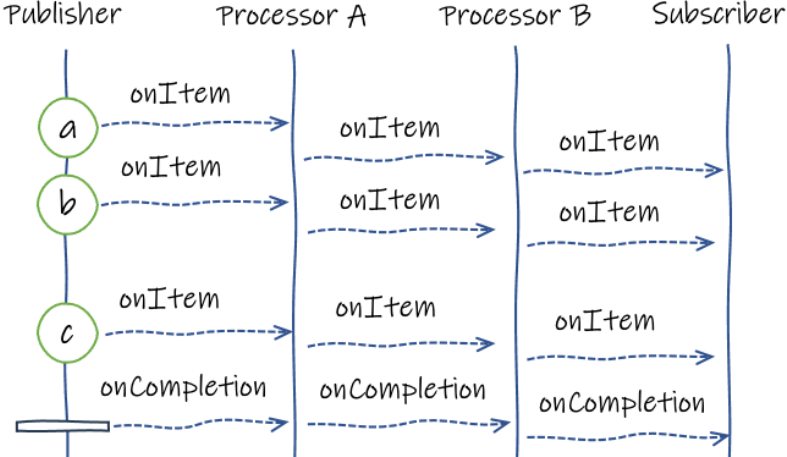
\includegraphics[width=0.9\textwidth]{EventFlow}
	\caption{Exemplarische Abbildung eines Event Flow in der Reactive Programming-Bibliothek Mutiny \parencite{MutinyEventFlow}}
	\label{fig:eventflow_mutiny}
\end{figure}

Reaktive Programmierung verinnerlicht das Konzept von nicht-blockierender bzw. asynchroner Ein- und Ausgabe (I/O).
Dabei wird, statt wie bei synchroner bzw. blockierender Ein- und Ausgabe die restliche Ausführung des Programms
zu blockieren bis die Datenübertragung abgeschlossen ist, nach dem Start der Übertragung bereits begonnen die Teile des
Programms auszuführen, die nicht von dem Ergebnis der I/O Operation abhängen.

\begin{lstlisting}[caption=Pseudocode Nonblocking I/O (NIO), captionpos=b, label=lst:NIO_Pseudocode]
NonBlockingDatabaseRequest().subscribe(print("req finished"))
NonBlockingDatabaseRequest2().subscribe(print("req 2 finished"))
print("hello world")
\end{lstlisting}
In Listing \ref{lst:NIO_Pseudocode} kann durchaus zuerst \verb|hello world| ausgegeben werden, da die gestarteten Datenbank-Anfragen die
restliche Programmausführung nicht blockieren. Wenn statt \verb|hello world| versucht würde, die Ergebnisse einer der Datenbank-Abfragen
darzustellen wäre das Ergebnis in der Regel eine Exception oder \verb|null|, da die Anfragen zur Zeit der Ausführung von Zeile 3 noch nicht notwendigerweise
abgeschlossen sind. Das ist ein sehr weit verbreiter Fehler beim Arbeiten mit asynchronen, nicht-blockierenden Funktionen.

\subsection{Vorteile und Nachteile}
\label{subsec:vorteile_nachteile}

Die Vorteile der Nutzung von einigen wenigen \verb|kernel threads| als \verb|IO Threads| gegenüber eines ganzen Threadpools
an \verb|kernel threads|, um einen \verb|kernel thread| an jede HTTP-Anfrage zu binden, liegen insbesondere in den Antwortszeiten bei
hoher Last und dem Ressourcenverbrauch.
Umso weniger \verb|kernel threads| gleichzeitig aktiv sind, umso weniger Threadwechsel auf Betriebssystemebene
gibt es auch pro CPU-Kern, wodurch die Antwortzeiten von Anwendungen wesentlich besser mit der Erhöhung der Last skalieren können,
da Threadwechsel nicht mehr der limitierende Faktor sind und jeder \verb|IO Thread| wesentlich mehr CPU-Rechenzeit nutzen kann.
Darüber hinaus sinkt auch der allokierte Speicher deutlich
\footnote{Eine 64 Bit-JVM reserviert auf Linux-und Solaris-Systemen standardmäßig 1 MB Speicher für den Threadstack eines Threads}
und der Grad der Parallellität wird nicht mehr von der Anzahl der verfübaren Threads begrenzt.

Die Umstellung auf das reaktive Programmierparadigma erfordert allerdings eine Änderung in der Denk- und Herangehensweise in der
Entwicklung von Softwarekomponenten. Denn reaktive Komponenten haben in der Regel keinen Zustand,
sondern reagieren lediglich auf interne Änderungen in den zugrundeliegenden Datenströmen.
Die bisherigen Programmabläufe müssten daher als reaktive Pipelines neu konstruiert werden.

Darüber hinaus ist reaktiver Code schwieriger zu debuggen und zu testen als imperativer Code, denn die Programmlogik die in den einzelnen Operatoren
der \verb|Pipes| einer \verb|Pipeline| aufgerufen wird, besteht in der Regel aus anynomen Funktionen und ist daher schwierig im Stack Trace einer
\verb|Pipeline| zurückzuverfolgen.
Während \verb|Event Flows| bei kleinen Pipelines noch zu überblicken sind, können komplexe Pipelines, die sich über die ganze Anwendung erstrecken,
schnell unklar werden.
Reaktive Programmierung ist zudem mit einer steilen Lernkurve verbunden. Dies liegt unter Anderem an dem aktuellen Interesse an skalierenden
Anwendungen und der damit oftmals einhergehenden falschen Verwendung von Begriffen und der Überladung des Begriffs \verb|Reactive Programming|.
Außerdem gibt es, Stand dieser Arbeit, kaum allgemeine, Hersteller
-unabhängige Fachliteratur zum Programmierparadigma, wodurch sich viele verschiedenen Nomenklaturen und Vorgehensweisen der verschiedenen Anbieter von
Reaktive-Programming-Bibliotheken (siehe \ref{subsec:java_ökosystem}), die sich größtenteils vor dem \verb|Reactive Streams|-Standard entwickelt haben,
nicht klar voneinander abgrenzen.

Ein weiteres Problem besteht bei der Integration in bestehende Enterprise Anwendungen. Bibliotheken und Konzepte die Themen wie
Security, Transaktionen oder Tracing behandeln, führen oft immernoch blockierenden, threadgebundenen Code aus.
Jede Schicht einer Anwendung muss reaktiv konzipiert sein, da die Verarbeitung einer Anfrage, die blockierenden Code aus einer der
Schichten aufruft, ansonsten den ausführenden IO-Thread blockieren kann, wodurch dieser keine weiteren Anfragen bearbeiten kann und somit die gesamte Anwendung blockiert.

Die wesentlichen Vor-und Nachteile lassen sich wie folgt zusammenfassen:

Vorteile
\begin{itemize}
	\item Die Antwortenzeiten sind für eine hohe Last geringer, da deutlich weniger Threadwechsel gemacht werden müssen und jeder Thread
	      mehr Rechenzeit bekommt
	\item Der Speicherverbrauch ist geringer, da weniger Threads genutzt werden
	\item Der Grad der Parallellität ist nicht von der Anzahl der Threads begrenzt
\end{itemize}
Nachteile
\begin{itemize}
	\item Asynchroner Code ist schwieriger zu schreiben, lesen, testen und zu debuggen als imperativer Code
	\item Sehr aufwendig in bestehende klassische Enterprise-Anwendungen zu integrieren
	\item Reaktive Anwendungen müssen in jeder Schicht reaktiv sein (Transaktionen, Security, Datenbanktreiber)
	\item Blockierende I/O-Operationen führen zur Blockierung des IO-Threads und damit zur Blockierung der gesamten Anwendung
\end{itemize}

\subsection{Reaktive Datenströme}
\label{section:reaktive_datenströme}
In einer typischen asynchronen Verarbeitungskette von, potenziell unbegrenzten, Datenströmen
bestehend aus einem Sender und Empfänger bzw. Publisher und Subscriber kann es vorkommen,
dass der Sender Daten schneller an den Empfänger verschickt, als dieser sie verarbeiten kann.
Zwei naive Ansätze mit einer Überlastung des Empfängers umzugehen wären:
\begin{enumerate}
	\item Nur der Empfänger reagiert auf eine Überlast. Diese kann sich in einem Speicherüberlauf äußern oder, falls der Puffer des Empfängers eine Größenbeschränkung
	      hat, im Verlust der empfangenen Daten
	\item Der Sender begrenzt im vornherein die Datenmenge, die er an den Empfänger schickt. Da der Sender allerdings in der Regel nicht weiß wieviel der Empfänger
	      verarbeiten kann, sendet er entweder zuviel (es entsteht eine Überlast), oder er sendet zuwenig wodurch der Durchsatz geringer ist als nötig
\end{enumerate}\parencite{JavaSpektrum2015}
Die Lösung für dieses Problem wird \textit{Backpressure} genannt.
Dabei fordert der Empfänger die Daten entsprechend seiner Kapazitäten an, wodurch der Sender weiß wieviele Daten er maximal versenden darf.
Diese Mitteilung muss asynchron geschehen, da bei einer synchronen Kommunikation der Backpressure die Vorteile der asynchronen, reaktiven Datenverarbeitung
negiert würden.
Da große Anwendungen aus mehreren Schichten (bspw. Routing-Schicht, Persistenzschicht, Geschäftslogik) bestehen und somit zwischen
dem Sender und Empfänger mehrere Komponenten liegen können, muss jedes
Element der Verarbeitungskette nichtblockierendes, asynchrones Verhalten implementieren, da ansonsten der Rest der Kette blockiert würde.

Aus der Intention einen Standard für die asynchrone Verarbeitung von Datenströmen mit nicht-blockierender \textit{back pressure}
zu schaffen, ging die \textit{Reactive Streams}-Initiative hervor.
Innerhalb dieser Initiative haben sich mehrere Arbeitsgruppen gebildet, welche die grundlegenden Semantiken erarbeitet haben und
sie in Form einer eigenen Java-Spezifikation namens \textit{Reactive Streams}-API implementiert und veröffentlicht haben.\parencite{ReactiveStreams}
Diese API wurde anschließend in Java 9, als Schnittstelle namens \textit{Flow-API} dem JDK hinzugefügt.
Die \textit{Flow-API} des JDK entspricht der \textit{Reactive Streams} Spezifikation und stellt (nur) Interfaces zur Verfügung mit denen eine
asynchrone, nicht blockierende Verarbeitung von (unbegrenzten) Datenströmen mit \textit{back pressure} auf der JVM implementiert werden kann.
\parencite{OracleFlow}.
\footnote{Nicht zu Verwechseln mit den Java-Streams durch die Collection-API ab Java 8. Diese sind zur Auswertungszeit in ihrer Größe begrenzt und
	nach der Abarbeitung liegt statt eines Streams eine Collection vor}

\subsubsection{Java Flow-API}
\label{subsection:java_flow_api}
Die Flow-API fügt die, nicht instanziierbare, Klasse \verb|java.util.concurrent.Flow| hinzu. Sie enthält 4 Interfaces um das,
vom \textit{Reactive Streams}-Projekt standardisierte, beschriebene Publisher-Subscriber Model des Daten- bzw. Eventflusses
(siehe \ref{lst:eventflow_pseudocode} und \ref{fig:eventflow_mutiny}) mit \verb|backpressure|
von reaktiven Anwendungen auszudrücken:
\begin{enumerate}
	\item Publisher
	\item Subscriber
	\item Subscription
	\item Processor
\end{enumerate}

Die \verb|Flow|-Klasse erlaubt es Komponenten zu implementieren die Teil von reaktiven Pipelines sein können, in denen
\verb|Publisher| Elemente produzieren, die von einem oder mehr \verb|Subscriber| konsumiert werden. Die Beziehung zwischen einem
\verb|Publisher| und \verb|Subscriber| wird durch eine \verb|Subscription| abgebildet.
Während ein \verb|Publisher| theoretisch eine unbegrenzte Menge an Events liefern kann, wird er eingeschränkt durch den
\verb|Backpressure|-Mechanismus. Dadurch liefert der \verb|Publisher| immer nur soviele Elemente wie vom \verb|Subscriber| gefordert.
Der \verb|Publisher| erlaubt einem \verb|Subscriber| sich bei ihm zu registrieren um über die herausgegebenen Events informiert zu werden.
Die Kontrolle über den Fluss an Elementen (flow control), inklusive \verb|backpressure|, zwischen einem \verb|Publisher| und seinen \verb|Subscribern|
wird von der \verb|Subscription| verwaltet.
In Listing \ref{lst:java_flowapi} werden die 4 Interfaces der Flow-API dargestellt:
\begin{lstlisting}[language=java, caption=Die Klasse java.util.concurrent.Flow, captionpos=b, label=lst:java_flowapi]
@FunctionalInterface
public static interface Flow.Publisher<T> {
	public void subscribe( Flow.Subscriber<? super T> subscriber );
}
public static interface Flow.Subscriber<T> {
	public void onSubscribe( Flow.Subscription subscription );
	public void onNext( T item );
	public void onError( Throwable throwable );
	public void onComplete();
}
public static interface Flow.Subscription {
	public void request( long n );
	public void cancel();
}
public static interface Flow.Processor<T,R>
extends Flow.Subscriber<T>, Flow.Publisher<R> {
}
\end{lstlisting}\parencite[Kapitel 5.11]{JavaSE9StandardBibliothek}

Die vier \verb|Callback|-Methoden des \verb|Subscriber|-Interface werden vom \verb|Publisher| aufgerufen sobald eines der jeweiligen Events ausgelöst wird.
Die Events müssen dabei immer in der gleichen Reihenfolge veröffentlicht (und die jeweiligen Callback-Methoden ausgeführt) werden:
\begin{enumerate}
	\item onSubscribe
	\item onNext*
	\item (onError | onComplete)?
\end{enumerate}
Die Notation bedeutet, dass \verb|onSubscribe| immer als erstes aufgerufen werden muss, gefolgt von einer beliebigen Anzahl an
\verb|onNext|-Aufrufen. Dieser Eventstrom kann theoretisch ewig weitergehen, oder durch ein \verb|onComplete|-Aufruf beendet werden, welches
signalisiert das keine weiteren Elemente mehr vom \verb|Publisher| produziert werden.
Im Fehlerfall wird vom \verb|Publisher| das \verb|onError|-Callback aufgerufen.

Sobald sich ein \verb|Subscriber| bei einem \verb|Publisher| registriert, wird zuerst die \verb|onSubscribe|-Methode aufgerufen und dann ein
\verb|Subscription|-Objekt zurückgegeben. Ein \verb|Subscription|-Objekt wird nur von genau einem \verb|Subscriber| und einem \verb|Publisher| genutzt
und bildet die einzigartige Beziehung zwischen ihnen ab.

Der \verb|Subscriber| kann die erste Methode des \verb|Subscription|-Interfaces nutzen um den \verb|Publisher| zu informieren, dass er bereit
ist eine gegebene Anzahl an Events zu verarbeiten (backpressure). Mit der \verb|cancel|-Methode kann er die \verb|Subscription| abbrechen und dem \verb|Publisher|
somit mitteilen das er nicht länger Events erhalten will.
\parencite{JavaSEFlow}

Das \verb|Processor|-Interface erweitert \verb|Publisher| und \verb|Subscriber| ohne das weitere Methoden implementiert werden müssen.
Dieses Interface repräsentiert eine Transformation der Events, die durch den
reaktiven Datenstrom verarbeitet werden (siehe Listing \ref{lst:eventflow_pseudocode}).
Klassen die dieses Interface implementieren repräsentieren in der Regel die Operatoren einer Reactive Programming-Bibliothek.
Sobald ein \verb|Processor| ein Fehler erhält kann er sich entweder davon erholen oder direkt das onError-Signal an seinen
Downstream-Subscriber propagieren. Ein typischer Lebenszyklus eines reaktiven Datenstroms mit der Flow-API wird in
Abbildung \ref{fig:flow-api} gezeigt.
\begin{figure}[h]
	\centering
	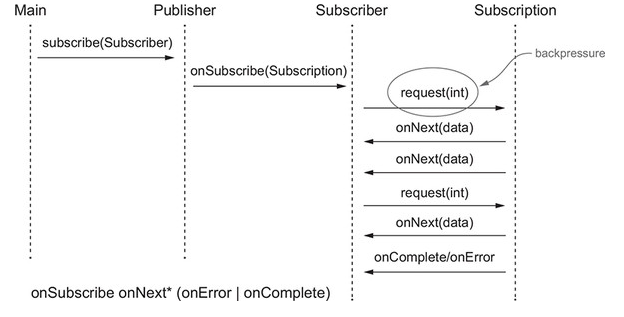
\includegraphics[width=0.9\textwidth]{flow-api_manning.PNG}
	\caption{Lebenszyklus eines reactive streams mit der Flow-API \parencite[Kapitel 17,  Figure 17.3]{JavaInAction}}
	\label{fig:flow-api}
\end{figure}
\newpage

\subsection{Reaktive Systeme}
\label{subsection:reaktive_systeme}
Anforderungen an große Softwaresysteme haben sich in den letzten Jahren stark verändert:
\begin{itemize}
	\item Antwortzeiten in Millisekunden statt im Sekundenbereich
	\item Datengrößen in Petabytes statt Gigabytes
	\item 100\% Verfügbarkeit statt stundenlange Wartungsarbeiten
	\item Deployment auf einer Vielzahl von Plattformen und cloud-basierten Clustern mit tausenden Multikernprozessoren
\end{itemize}

Unternehmen aus verschiedenen Bereichen haben sich voneinander unabhängig an diese Kriterien angepasst und Architekturmuster
erarbeitet, mit denen robuste, belastbare und flexible Softwaresysteme entwickelt werden können, die die modernen Anforderungen
erfüllen.

2014 wurde mit dem \verb|Reactive Manifesto| versucht diese Ansätze der Systemarchitektur in Form eines Manifests zusammenzuführen
und daraus allgemeingültige Systemattribute abzuleiten.

\subsubsection{Eigenschaften}
\label{subsubsec:reaktive_systeme_eigenschaften}
Laut des \verb|Reactive Manifesto| sind Systeme reaktiv wenn sie:
\begin{itemize}
	\item Reaktionsschnell
	\item Widerstandsfähig (gegen Fehler)
	\item Elastisch
	\item Nachrichtengesteuert
\end{itemize}
sind.
Solche Systeme sind, laut den Autoren, flexibler, stärker entkoppelt und würden besser skalieren als herkömmliche, nicht-reaktive Systeme.
Dies mache sie leichter zu entwickeln, zugänglicher für Veränderungen und deutlich fehlertoleranter.

Die Autoren definieren die genannten Systemeigenschaften wie folgt:

\paragraph{Reaktionsschnelligkeit}: Das System reagiert, falls überhaupt möglich, zeitgerecht. Reaktionsschnelligkeit ist dabei die Grundlage für Funktion und
Benutzbarkeit. Es ermöglicht das schnelle Erkennen und Behandeln von Fehlern, indem verlässliche, zeitliche Obergrenzen für die Antworten von
Komponenten innerhalb des Systems geschaffen werden. Sobald eine Komponente nicht innerhalb des Zeitfensters antwortet, wird dies als Fehler gewertet und kann
entsprechend behandelt werden.
Der Fokus von reaktionsschnellen Systemen liegt auf konsistenten und schnellen Antwortszeiten. Darüber hinaus schaffen sie
verlässliche Obergrenzen um eine konsistente Qualität zu erreichen.
Dieses Verhalten simplifiziert Fehlerbehandlung, und erhöht das Vertrauen der Benutzer bezüglich Interaktionen.

\paragraph{Widerstandsfähig/Fehlertolerant}: Das System bleibt auch bei Fehlern reaktionsschnell. Das gilt nicht nur geschäftskritische, hochverfügbare Systeme -
jedes System das nicht Fehlertolerant ist, wird nach Fehlern nicht mehr reaktionsfähig sein.
Widerstandsfähigkeit wird durch Replikation von Funktionalität bzw. Redundanz, Eingrenzung von Fehlern, Isolation von Komponenten und
Delegatieren von Verantwortung realisierbar.
Fehler werden innerhalb einer Komponente eingegrenzt und die Komponenten sind voneinander isoliert. Dadurch bleibt das Gesamtsystem stabil, selbst
wenn eine einzelne Komponente versagt.
Die Wiederherstellung jeder Komponente (self-healing) wird an eine andere (möglicherweise externe) Komponente deligiert, und
Hochverfügbarkeit der Komponenten wird, wo notwendig, durch Redundanz gewährleistet.

\paragraph{Elastisch}: Das System bleibt reaktionsschnell unter variierenden Arbeitslasten. Auf Änderungen der Arbeitslast wird durch das Replikation
das Anpassen der, durch Replikation, allokierten Ressourcen reagiert. Das impliziert ein Systemdesign das keine zentralen Performance-Bottlenecks oder
Reibunspunkte hat, damit Komponenten problemlos repliziert und die Last darauf verteilt werden kann.

Reaktive Systeme unterstützen prädiktive, skalierende Algorithmen zur Ressourcenberechnung,
indem Sie die Live-Messungen von Performance relevanten Systemmetriken als Eingabe nutzen.

\paragraph{Nachrichtengesteuert}: Reaktive Systeme basieren auf dem asynchronen, nichtblockierendem Austausch von Nachrichten, um die Komponenten voneinander
abzugrenzen und dadurch eine loose Kopplung, Isolation und eine transparente Lokalisierung der Komponenten zu ermöglichen.
Aufgrund dieser Abgrenzung werden Fehler als Nachrichten an andere Komponenten delegiert.
Der Ansatz jegliche Kommunikation der Komponenten durch das Übermitteln von Nachrichten zu implementieren erlaubt Elastizität,
indem er das Verteilen der Arbeitslast, und die Kontrolle der Datenströme durch das Überwachen der Nachrichtenwarteschlangen zur Laufzeit
(\textit{message queues}) und, falls nötig, Anwenden von \textit{back pressure}, erlaubt.
Ortsunabhängigkeit bedeutet, dass Code und Semantik des Programms nicht davon abhängen, ob dessen Teile auf demselben Computer
oder verteilt über ein Netzwerk ausgeführt werden.
Nicht-blockierende nachrichtenorientierte Systeme erlauben eine effiziente Verwendung von Ressourcen, da Komponenten beim Ausbleiben von
Nachrichten vollständig inaktiv bleiben können, und sich nicht regelmäßig über neue Nachrichten informieren müssen.\parencite{ReactiveSystems}

Im Gegensatz zu Events haben Nachrichten immer ein klar definiertes Ziel.
Das bedeutet, dass sich ein ereignisgesteuertes System- oder eine Systemkomponente auf adressierbare Event-Quellen konzentriert,
während ein nachrichtengesteuertes System auf adressierbaren Empfängern basiert.

In Abbildung \ref{fig:reactive-traits} wird das Zusammenspiel der Eigenschaften eines reaktiven Systems dargestellt.

\begin{figure}[h]
	\centering
	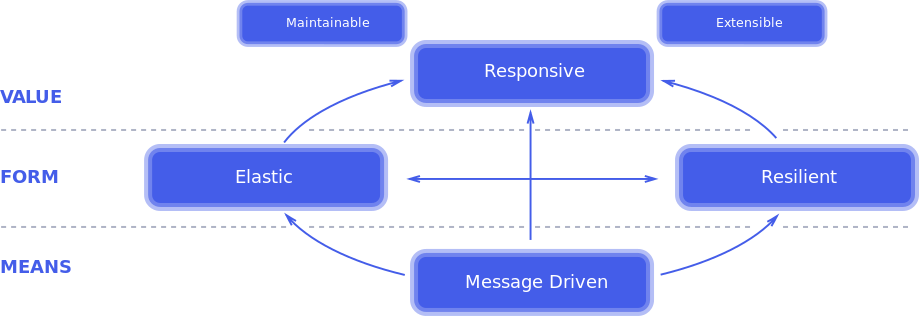
\includegraphics[width=0.9\textwidth]{reactive-traits}
	\caption{Zusammenspiel der Eigenschaften eines reaktiven Systems \parencite{ReactiveSystems}}
	\label{fig:reactive-traits}
\end{figure}

\subsubsection{Abgrenzung zu reaktiver Programmierung}
\label{subsubsection:abgrenzung_reaktive_programmierung}
Aufgrund der steigenden Popularität von reaktiven Anwendungen ist der Begriff \verb|reaktiv| im Kontext der Softwareentwicklung
überladen und unterscheidet nicht zwischen \linebreak\verb|Reaktiver Programmierung| und \verb|Reaktiven Systemen|.

\verb|Reaktive Programmierung| ist eine ideale Technik zur Abbildung der internen Logik innerhalb einer Komponente, in Form von Transformationen
auf Datenströmen, um sowohl Performance, Ressourceneffizienz und Code-Verständlichkeit zu optimieren.

\verb|Reaktive Systeme| sind hingegen eine Menge von architektonischen Prinzipien, die die verteilte Kommunikation hervorheben und
Ansätze zur Realisierung von Fehlertoleranz und Elastizität liefern.

Ein gängiges Problem bei ausschließlicher Nutzung von \verb|Reaktiver Programmierung| besteht darin, dass die enge Kopplung
zwischen Verarbeitungsschritten (Transformationen) in einem eventgesteuerten Programm die geforderte Fehlertoleranz eines reaktiven Systems
schwer zu erreichen macht.
Die Transformationsketten bzw. \verb|Pipelines| sind kurzlebig und die Operatoren und Callback-Methoden innerhalb der \verb|Pipes|
sind anonym, also nicht adressierbar.

Das bedeutet, dass sowohl Erfolg, als auch Misserfolg bzw. Fehler direkt behandelt werden, ohne andere Komponenten darüber zu informieren.
Dieser Mangel an Adressierbarkeit erschwert die Wiederherstellung einzelner Phasen, da unklar ist, wo beziehungsweise ob Ausnahmen
propagiert werden sollten. Infolgedessen sind Fehler an kurzlebige Client-Anfragen und nicht an den
Gesamtzustand der Komponente gebunden – wenn eine der Phasen in der \verb|Pipeline| fehlschlägt, muss die gesamte \verb|Pipeline| neu
gestartet und der Client benachrichtigt werden. Dies steht im Gegensatz zu einem nachrichtengesteuerten reaktiven System, das
die Fähigkeit zur Wiederherstellung von Komponenten besitzt, ohne dass der Client benachrichtigt werden muss.

Ein weiterer Kontrast zum Ansatz eines reaktiven Systems ist, dass rein reaktive Programmierung zwar eine zeitliche Entkopplung,
aber keine räumliche Entkopplung ermöglicht. Zeitliche Entkopplung erlaubt gleichzeitige Verarbeitung, während räumliche Entkopplung
die Verteilung auf mehrere Systemkomponenten erlaubt. Dadurch können nicht nur statische, sondern auch dynamische Topologien
realisiert werden, was für die Elastizität eines reaktiven Systems essentiell ist.

Insgesamt ist \verb|reaktives Programmieren| eine sehr nützliche Technik, die in einer reaktiven Architektur genutzt werden kann.
Das Implementieren von Datenflüssen durch asynchrone und nichtblockierende Ausführung innerhalb eines Services bildet
die Basis eines reaktiven Systems, mehrere reaktive Services bilden aber noch kein reaktives System.

Sobald mehrere Services in einem reaktiven System miteinander arbeiten sollen, müssen unter Anderem Funktionalitäten wie
Datenkonsistenz, Serviceübergreifende Kommunikation, Versionierung, Orchestrierung, Fehlermanagement und Trennung von Verantwortlichkeiten
berücksichtigt werden.

\subsection{Java Ökosystem}
\label{subsec:java_ökosystem}
Im Java Ökosystem gibt es eine Vielzahl an Libraries und Frameworks mit denen
\verb|Reaktive Programmierung| und \verb|Reaktive Systeme| umgesetzt werden können.
Um in Java einzelne, asynchrone Prozesse zu implementieren, wird vom JDK die Future-API zur Verfügung gestellt.\parencite{OracleFuture}
Für die Verarbeitung von asynchronen (unbegrenzten) Datenströmen gibt es die Interfaces der Flow-API (siehe \ref{subsection:java_flow_api}).
\parencite{OracleFlow}

Im Folgenden wird ein Überblick über die Vielzahl an Bibliotheken und Frameworks gegeben.

\subsubsection{Reaktive Datenströme - Bibliotheken}
\label{subsubsec:reactive_streams}
Da die Flow-API lediglich Interfaces bereitstellt, gibt es mehrere Implementierungen von \verb|Reaktiven Datenströmen|.
Zu den populärsten Bibliotheken zählen:
\begin{itemize}
	\item RxJava
	\item Spring Webflux
	\item Mutiny
\end{itemize}
Jedes Projekt unterscheidet sich dabei in den verwendeten Klassen - und Operatoren um die \verb|reactive streams|-Spezifikation
beziehungsweise die \verb|Flow-API| des JDK zu implementieren.
\begin{itemize}
	\item RxJava\footnote{Implementiert die Flow-API erst seit Version 2} - Flowable, Observable \parencite{RxJava}
	\item Project Reactor - Flux, Mono \parencite{ProjectReactor}
	\item Mutiny - Multi, Uni \parencite{Mutiny}
\end{itemize}

Die Bibliotheken sind interoperabel, da sie die \verb|reactive streams|-Spezifikation in Java mithilfe der \verb|Flow-API|
implementieren \footnote{Und damit auch \textit{back pressure}} und Converter-Klassen anbieten.

\subsubsection{Reaktive Systeme - Toolkits}
\label{subsubsec:reaktive_systeme}
Für die Entwicklung von reaktiven Systemen bieten sich mehrere Toolkits an.
Sie implementieren bereits Mechanismen wie Messaging, Event Loops,
nichtblockierende Netzwerkanwendungen und Dateizugriffe, sowie umfangreiche Funktionen für Webanwendungen.
Zu den populärsten gehören:
\begin{itemize}
	\item Eclipse Vert.x
	\item Akka
	\item Reactor-Netty
\end{itemize}\parencite{Vert.x, Akka, ProjectReactor}
Sowohl \verb|Eclipse Vert.x| als auch Reactor-Netty nutzen dabei \verb|Netty|
(siehe \ref{subsubsec:reactor_pattern}) als Low-Level Framework für \verb|Nonblocking I/O|.
Da das in dieser Arbeit verwendete Anwendungsframework \verb|Quarkus| auf \verb|Eclipse Vert.x| basiert, wird Vert.x im Folgenden genauer beschrieben:

\paragraph{Eclipse Vert.x}
Vert.x ist ein Toolkit für das Entwickeln von reaktiven Anwendungen auf der JVM und wird unter dem Dach der herstellerneutralen Eclipse Foundation entwickelt.
Da es sich nicht um ein Framework handelt, gibt es keine vordefinierte Grundlage für Anwendungen und dadurch kann es auch in bestehende Projekte
integriert werden.
Der Kern des Toolkits \verb|vertx-core| stellt APIs für asynchrones Programmieren, \verb|Nonblocking I/O|, Streaming und Zugriff zu
Netzwerkprokollen wie TCP, UDP, DNS HTTP oder WebSockets.
\begin{figure}[h]
	\centering
	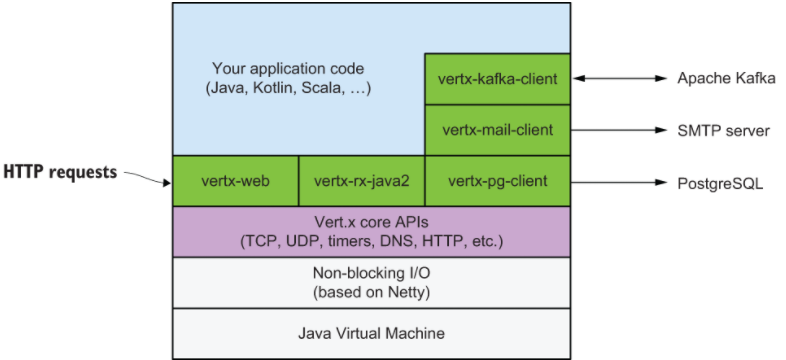
\includegraphics[width=1.0\textwidth]{vertx}
	\caption{Vert.x Struktur \parencite{Ponge2020}}
	\label{fig:vertx}
\end{figure}

Für die räumliche Entkopplung eines reaktiven Systems bietet Vert.x einen \verb|Event Bus|.
Der \verb|Event Bus| stellt ein verteiltes Peer-To-Peer Nachrichten System dar, welches sich über mehrere Serverknoten ersteckt.
Damit können verschiedene Komponenten eines Systems, unabhängig von der genutzten Programmiersprache, durch eindeutige Addressierung miteinander kommunizieren.
Auf jede Adresse können sich, ganz nach dem \verb|Publish-Subscribe|-Modell, mehrere Subscriber registrieren. Sobald Nachrichten an eine
Adresse veröffentlicht (published) werden, werden diese an jeden \verb|Subscriber| weitergeleitet.

Für die Resilienz eines reaktiven Systems verfügt Vert.x über einen Hochverfügbarkeits-Modus (high availablity, HA).
Dabei wird im Falle des Versagens einer Vert.x-Instanz die Anwendung auf eine andere Instanz aus einem Cluster redeployed.
Darüber hinaus wird im Falle des Ausfalls einer Komponente durch einen Circuit Breaker vermieden, dass weitere Anfragen an diese
Komponente getätigt werden.\newline

Eine Implementierung des \verb|Reactor|-Pattern nutzt standardmäßig einen einzigen \verb|Event loop|-Thread, der in einer Schleife alle
Events an die jeweils registrierten Event-Handler liefert.
Da durch einen einzigen \verb|Event loop|-Thread allerdings zu jeder Zeit auch nur ein CPU-Kern genutzt wird, kann
eine solche Implementierung Mehrkern-CPUs nur nutzen, indem mehrere Prozesse gestartet und verwaltet werden.

Statt einer einzigen Event Loop hält jede Vertx-Instanz mehrere, abhängig von der Anzahl der verfügbaren CPU-Kerne\footnote{1 Thread pro logischem CPU-Kern},
\verb|Event loop|-Threads. Diese Threads werden aus einem im vornherein erzeugten \verb|Event loop thread pool| entnommen.
\footnote{Die Größe des \textit{event loop thread pools} kann auch manuell überschrieben werden}

Um dieses Pattern vom Single Threaded Reactor-Pattern zu unterscheiden, wird es in der Vert.x-Dokumentation als \verb|Multi-Reactor Pattern| bezeichnet.
\parencite{Vert.xDocs}  \newline

Im Falle dass eine Event Loop durch \verb|Blocking I/O| blockiert würde, wird die Operation stattdessen auf einen
Worker Thread, aus einen im vornherein erzeugten \verb|Worker thread pool|, abgewickelt. Dieser Prozess bezeichnet \verb|Vert.x| als \verb|Dispatching|.
Dadurch entstehen natürlich wieder Threadwechsel, ermöglichen aber die Nutzung von Vert.x in bestehenden Projekten, die nicht komplett
auf \verb|Nonblocking I/O| basieren\parencite[Seite 2]{VertxArticle}.
Vert.x führt also zwei Thread Pools mit \verb|Kernel-Threads|, einen für \verb|Event loop threads|, dessen Größe der Anzahl der logischen CPUs entspricht,
und einen für \verb|Worker threads|, auf dem die Operationen abgearbeitet werden die die \verb|Event loop threads| blockieren würden.
\parencite{Vert.xOptions}

\subsubsection{Frameworks}
\label{subsubsec:frameworks}
Um komplette Web-Applikationen zu implementieren bietet sich der Gebrauch von Frameworks an, die Entwicklern viele grundlegende Architekturentscheidungen
abnehmen und bereits vorgefertigte Lösungen für Themen wie Authenfizierung, Routing, \Gls{ormg}(*), Security und Serialisierung anbieten oder
Lösungen von Drittanbietern integrieren und vorkonfigurieren.
Um reaktive Anwendungen und Systeme mit mehreren Services sinnvoll zu nutzen, ist es notwendig dass jede, für die Abarbeitung eines Requests relevante,
Anwendungsschicht und Komponente auch reaktiv ist und \verb|Nonblocking I/O| benutzt, sowie eine API bietet auf der
sich Event-Handler bzw. Subscriber registrieren können.

Die populärsten Frameworks mit einem komplett reaktiven Stack sind dabei:

\begin{itemize}
	\item Spring WebFlux
	\item Quarkus
\end{itemize}

Spring WebFlux nutzt dabei \verb|Project Reactor| und Quarkus \verb|Vert.x| als reaktive Engine. \parencite{QuarkusReactiveGettingStarted}
Da die exemplarischen Anwendungen dieser Arbeit (siehe Kapitel \ref{section:vergleich_reaktiv_imperativ}) das Quarkus-Framework nutzen, wird dies
im Folgenden genauer beschrieben:
\paragraph{Quarkus und native image}

Bei dem, in dieser Arbeit verwendeten, Framework \verb|Quarkus| handelt es sich laut Hersteller Red Hat, um ein
benutzerfreundliches, auf Entwickler abgestimmtes Java Framework, welches für Container-, Cloud- und Serverless-Umgebungen optimiert ist und nur wenig
Konfiguration benötigt, sowie nur die besten und hochwertigsten Java-Bibliotheken und Standards nutzt.
Dabei können die Anwendungen sowohl auf einer JVM (JVM mode) laufen, als auch, durch native Kompilierung mit vollständigem Stack,
als nativ ausführbare Anwendung: dem \textit{native image} (native mode).

Dafür nutzt Quarkus eine, von Oracle entwickelte, Technologie namens \verb|GraalVM|.
Dabei handelt es sich um eine polyglotte, virtuelle Maschine und Laufzeitumgebung die auf dem OpenJDK basiert, und über
JVMCI \footnote{Java Virtual Machine Compiler Interface} den C2-Compiler der zugrundeliegenden HotSpot-JVM durch den
polyglotten Graal Compiler ersetzt.\parencite{GraalVM}
Beim C2-Compiler handelt es sich dabei um einen aggressiv optimierenden \verb|just-in-time| (JIT) Compiler für Serveranwendungen, bei denen es nicht auf
schnelle Startzeiten und geringen Ressourcenverbrauch, sondern auf höchsten Durchsatz ankommt.
Dabei wird der unoptimierte Bytecode während der Laufzeit in Maschinencode umgesetzt und ausgeführt. Sobald eine Methode hinreichend oft
ausgeführt wurde, daher auch als \verb|JIT Warm up| bezeichnet, und der Profiler genügend Informationen gesammelt hat, kann der JIT-Compiler
sie entsprechend optimieren, bevor sie in Maschinencode umgesetzt wird.
Der Graal Compiler kann sowohl als JIT-Compiler genutzt werden (JVM mode), als auch als AOT-Compiler (native mode).\newline

Um ein \verb|native image| zu erstellen, wird mithilfe des GraalVM-Compilers vor der Kompilierung, also \verb|ahead-of-time| (AOT), der Anwendung in Maschinencode
ermittelt welche möglichen Pfade das Programm bei einem gegebenen Klassenpfad durchlaufen kann. Da dadurch nur die tatsächlich benötigten Klassen
kompiliert werden sind Programme, die mit \verb|native image| erstellt wurden, um einige Größenordnungen kleiner als die Summe aus
JDK und den benötigten Bibliotheken.
Allerdings dauert der Vorgang aufgrund der umfassenden Analyse wesentlich länger als die Übersetzung in Bytecode mit \verb|javac| oder \verb|clang|.
Damit Entwickler sich bei Java Anwendungen auch weiterhin nicht um Speicher-und Threadverwaltung kümmern müssen, wird die \verb|SubstrateVM|, eine
leichtgewichtige virtuelle Maschine, in das \verb|native image| hineinkompiliert.
Sie stellt Laufzeitkomponenten wie den Garbage Collector und den Thread Scheduler bereit.

Die Analyse vor dem Kompilieren erfolgt unter der \verb|closed world|-Annahme. Dabei wird angenommen das jeglicher Code der zur Laufzeit des Programms
erreichbar ist, zur Build-Time des \verb|native image| bekannt sein muss. Dadurch verursachen jegliche Java-Features deren Ergebnis nicht exakt
zur Build-Time voraussbestimmbar ist, wie beispielsweise Reflection oder statische Initialisierung mit Datumswerten, Probleme für die Ahead-of-Time-Übersetzung.

Um dem Compiler die notwendigen Informationen zur Unterstützung von Reflection mitzuteilen, können
diese über Konfigurationsdateien oder programmatisch über die GraalVM- und SubstrateVM-API hinterlegt werden.
Dadurch können auch Anwendungen und Libraries die starken Gebrauch von Reflection machen wie beispielsweise Hibernate, Netty oder Tomcat
so angepasst werden, dass sie in einem \verb|native image| genutzt werden können.
\parencite{GraalVMNativeImage}
Darüber hinaus verspricht Quarkus, mit seiner Container-first-Philosophie durch \textit{native images} bis zu 300 Mal schnellere Startzeiten
und nur ein Zehntel des Speicherbedarfs im Vergleich zu traditionellen Java-Frameworks wie Spring Boot, wodurch es eine signifikante Reduzierung
der benötigten Ressourcen und Kosten, im Gegensatz zu einer herkömmlichen Java-Anwendung, im Cloud-Umfeld darstellt.
\parencite{RedHatQuarkusInfografik}
Allerdings ist der maximal, mögliche Durchsatz (noch) deutlich niedriger gegenüber Anwendungen im \verb|JVM-Mode| , da auf einige adaptive
Laufzeitoptimierungen, wie JIT-Compiling, verzichtet wird.

Des Weiteren erlaubt Quarkus die Kombination von blockierendem und nicht blockierendem, reaktiven Code.
Dabei wird der Dispatching-Mechanismus von \verb|Vert.x| genutzt (siehe \ref{subsubsec:reaktive_systeme}), sobald also eine
\verb|Blocking I/O|-Operation aufgerufen wird, wird diese auf einem \verb|Worker thread| abgewickelt, statt die \verb|Event Loop|, und damit den
gesamten \verb|Event loop thread| bzw. \verb|IO thread|, zu blockieren.
Für die reaktive Programmierung bietet Quarkus die bereits genannte Bibliothek \verb|Mutiny| an.\parencite{Quarkus}

\subsection{Alternativen}
\label{subsec:alternativen}
In Java 1.1 wurden Threads als sog. \textit{Green Threads} implementiert. Dabei wurde die Möglichkeit Threads vom Betriebssystem, also \verb|Kernel threads|,
verwalten zu lassen gar nicht genutzt.
\textit{Green threads} waren als \textit{user threads} implementiert \footnote{Auch als \textit{Fiber} oder \textit{virtual thread} bezeichnet},
dabei ist die Funktionalität
nicht im Kernel implementiert, sondern in einer Programmbibliothek im \textit{Userspace}.
Da sich das Betriebssystem nicht um das Scheduling von \textit{user threads} kümmert
\footnote{Da es diese garnicht kennt, da Sie keine kernel threads}, wurde dies über einen eigenen Scheduling-Algorithmus der JVM
geregelt.\parencite{Oracle2010}
Ein \textit{green thread} existiert lediglich als Objekt innerhalb der JVM, und durch die virtuelle Speicherverwaltung entfallen somit
die aufwändigen Betriebssystemaufrufe beim
Erstellen eines Threads, sowie bei Thread- bzw. Kontextwechseln, denn der ausführende Main-Thread bleibt gleich.

Die Threadwechsel der \textit{user-threads} erfolgten ausschließlich innerhalb des Main-Threads, weswegen keine echte Parallelität realisiert werden konnte,
da immer nur ein Prozessorkern genutzt wurde.
Während der Vorteil dieses Modells darin lag, dass es keine 'echten' parallelen Zugriffe auf eine Resource innerhalb des JVM-Prozesses geben konnte
und die Synchronisation von Datenzugriffen daher leicht war, überwog schließlich der Umstand, dass keine Nutzung von mehreren Prozessorkernen
durch Multithreading möglich war, weswegen \textit{Green Threads} ab Java 1.3 zugunsten von \textit{native threads} entfernt wurden.

Mit dem OpenJDK Projekt \textit{Project Loom} ist die Idee von \textit{Green threads}
wieder aufgegriffen worden, allerdings nun als Ergänzung (statt Alternative) zu \textit{native threads}.
Statt alle virtuellen Threads auf dem nativen Main-Thread auszuführen, werden diese von einer geringen Anzahl an nativen \textit{worker threads},
die als Carrier eingesetzt werden, ausgeführt.
Deren Anzahl ist so gewählt, dass alle CPU Kerne durch Multithreading dauerhaft benutzt werden können
\footnote{In der Praxis laufen natürlich noch andere Prozesse auf dem Server, deren Threads auch ausgeführt werden müssen.}
, aber so wenig Kontextwechsel wie möglich ausgeführt werden müssen.\parencite{Oracle2021}
\footnote{Im Idealfall würde auf jedem CPU Kern ein \textit{worker thread} laufen,	ohne jemals einen Thread- bzw. Kontextwechsel zu machen.}
Während ein nativer Thread in einer 64 Bit JVM auf Linux-Systemen standardmäßig 1 MB für den Threadstack reserviert
und zusätzlich noch Metadaten abspeichert, ist ein virtueller Thread
lediglich ein Objekt im virtuellen Speicher der JVM und benötigt sehr wenig Resourcen (da er ja im Hintergrund von einem
nativen Thread abgearbeitet wird).
Aus diesem Grund können durchaus mehrere Millionen virtueller Threads erzeugt werden (bei entsprechend allokierten Heap-Speicher der JVM), wohingegen
die Erstellung von 10.000 nativen Threads entweder den allokierten Speicher weit überschreitet (wodurch der JVM-Prozess abstürzt) oder die Threadgrenze
des Betriebssystems überschreitet.

Sobald ein virtueller Thread nun eine blockierende I/O Operation ausführt führt die Laufzeitumgebung automatisch einen
virtuellen Threadwechsel (siehe Kapitel \ref{subsubsec:threadwechsel}) durch und ermöglicht dem nativen Thread währendessen einen
anderen virtuellen Thread auszuführen.

Das große Versprechen des Projektes ist außerdem, das Entwickler keine asynchronen Programmierparadigmen (wie u.A. \textit{Reactive Programming})
nutzen müssen um die beschriebenen virtuellen Threads (und die damit einhergehenden wesentlichen Performanceverbesserungen) nutzen zu können.
Um dieses Versprechen zu halten werden virtuelle Threads, statt als Bibliothek eines Drittanbieters, in Form einer eigenen JDK Version bereitgestellt.
In dieser Version wurden viele Teile der Standardbibliothek die mit I/O-Operationen arbeiten so angepasst, dass virtuelle Threads statt native Threads
genutzt werden. Auf diese Weise können I/O-Operationen, wie beispielsweise der Aufruf einer Netzwerkfunktionalität, ohne Änderungen am Programm,
die virtuellen Threads nutzen und blockieren den darunterliegenden nativen Thread nicht mehr.

Jüngere Programmiersprachen wie Kotlin und Golang benutzen bereits virtuelle statt nativer Threads
für ihre Threading-Abstraktion \verb|coroutines|. \parencite{KotlinCoroutines, GoCoroutines}